\documentclass[10pt,a4paper,table]{article}
	
	\usepackage{amsmath,amssymb,amsthm,mathtools,amsfonts}
	\usepackage{breqn}
	\usepackage[utf8]{inputenc}
	\usepackage[danish]{babel}
	\usepackage[T1]{fontenc}
	
	%%%%%%%%%%%%%%%%%%%%%%%%%%%%%%%%%%%%%%%%%%%%%%%%%%%%%%%%%%%%%%%%%%%%%%%%%%%%%% Fonts
	
	\usepackage{fontspec}
	\setmainfont{Times New Roman}
	\newfontfamily\garamond[Numbers=OldStyle]{EB Garamond}
	\newfontfamily\plantin[Numbers=OldStyle]{Plantin MT Pro}
	\newfontfamily\wal{Walbaum Com}
	\newfontfamily\klav{Klavika}
	\newfontfamily\klavl{Klavika light}
	\newfontfamily\quotefont[Ligatures=TeX]{Linux Libertine O}
	\newfontfamily\vest{TRY Vesterbro Regular}
	\newfontfamily\vestb{TRY Vesterbro Poster}
	\newfontfamily\overp{Overpass}
	
	%%%%%%%%%%%%%%%%%%%%%%%%%%%%%%%%%%%%%%%%%%%%%%%%%%%%%%%%%%%%%%%%%%%%%%%%%%%%%% Colors
	
	\usepackage{xcolor}
	
	\definecolor{frbblue}{RGB}{47, 88, 109}
	\definecolor{hgred}{RGB}{140, 10, 10}
	\definecolor{frbgreenl}{RGB}{162, 202, 137}
	\definecolor{frbgreen}{RGB}{28, 85, 66}
	\definecolor{frbgrey}{RGB}{243, 245, 242}
	
	%%%%%%%%%%%%%%%%%%%%%%%%%%%%%%%%%%%%%%%%%%%%%%%%%%%%%%%%%%%%%%%%%%%%%%%%%%%%%% Other Graphics
	
	\usepackage{graphicx}
	\graphicspath{{../img/}}
	\usepackage{tikz}
	\usepackage{placeins}
	\usepackage{subcaption}
  \usepackage{float}
	
	\usepackage[pdfborder={0 0 0}]{hyperref} %% Ingen firkant rundt om referencer

	\usepackage{multicol}
	\usepackage{cellspace}
		\setlength\cellspacetoplimit{100pt}
		\setlength\cellspacebottomlimit{100pt}
	\usepackage{tabularx}
		\newcolumntype{b}{>{\hsize=\hsize}>{\centering\arraybackslash}X}
	\usepackage{siunitx}
	\usepackage{cellspace}
		\setlength\cellspacetoplimit{4pt}
		\setlength\cellspacebottomlimit{4pt}
	
	\usepackage{enumitem}% better controls with enumerating
	\usepackage{wrapfig}
	\usepackage{caption}
	%\usepackage{dirtytalk}
	%\usepackage{tasks}
	\usepackage{titlesec}

	\setlength{\parskip}{0.5\baselineskip}
	\setlength{\parindent}{0cm}
	\setlist[enumerate]{label=\alph*),left=20pt}
	%\setlist[enumerate]{leftmargin=\parindent}
	%\setlist[enumerate]{nosep}
	
	
	%%%%%%%%%%%%%%%%%%%%%%%%%%%%%%%%%%%%%%%%%%%%%%%%%%%%%%%%%%%%%%%%%%%%%%%%%%%%%% New commands
	
	\newcommand\svar[1]{\color{red}{#1}\color{black}}
	
	\usepackage[h]{esvect}
	\newcommand{\twvect}[2]{\ensuremath{\begin{pmatrix}#1\\#2\end{pmatrix}}}
	
	\newcommand*\quotesize{20}
	\newcommand*{\openquote}
		{\tikz[remember picture,overlay,xshift=-3ex,yshift=-0ex]
			\node (OQ) {\quotefont\fontsize{\quotesize}{\quotesize}\selectfont``};\kern0pt}

	\newcommand*{\closequote}[1]
		{\tikz[remember picture,overlay,xshift=2ex,yshift={#1}]
			\node (CQ) {\quotefont\fontsize{\quotesize}{\quotesize}\selectfont''};}
			
	\newcommand{\qm}[1]{``#1''}
	\newcommand{\iquote}[1]{\begin{quote}\itshape \openquote#1\hfill\closequote{0ex} \end{quote}}
	
	%%%%%%%%%%%%%%%%%%%%%%%%%%%%%%%%%%%%%%%%%%%%%%%%%%%%%%%%%%%%%%%%%%%%%%%%%%%%%% Sections
	\usepackage{chngcntr}
	
	\renewcommand\thesection{\arabic{section}}

	\titleformat{\section}[block] 
  		{\flushright\overp\Large\color{frbgreen}}    % format for whole title
  		{}                           % no separate label (empty)
  		{0pt}                        % spacing between label and title
		{DELPRØVE \thesection}       % prepend "Delprøve <number>"
		[{\color{frbgreenl}\vspace{-1em}\hspace*{-0.165\linewidth}\rule{\dimexpr1.165\linewidth\relax}{0.4pt}\kern1mm}]
	
	\counterwithout{subsection}{section}
	\renewcommand\thesubsection{Opgave \arabic{subsection}}
	\titleformat{\subsection}[leftmargin]{\bfseries}{}{0pt}{\hspace{-5em}\thesubsection}
	
	%%%%%%%%%%%%%%%%%%%%%%%%%%%%%%%%%%%%%%%%%%%%%%%%%%%%%%%%%%%%%%%%%%%%%%%%%%%%%% Header & Footer
	
	\usepackage{bigfoot}
	\DeclareNewFootnote{a}
		\renewcommand{\thefootnotea}{\fnsymbol{footnotea}}
			\newcommand{\footnotes}[1]{\footnotea[2]{#1}} % here you can specify what symbol you want in footnotes
			\MakePerPage{footnotes}
	
		\usepackage{fancyhdr}
	\fancypagestyle{plain}{%
		\setlength{\headheight}{60pt}%
		\setlength{\headsep}{0pt}
		\fancyhf{}% No header/footer
		\renewcommand{\footrulewidth}{0pt}% No footer rule
		\renewcommand\headrule{
			\centerline{\begin{minipage}{1\textwidth}
				\color{frbblue}\hrule width \hsize \kern 1mm \hrule width \hsize height 2pt \vspace{4em}
			\end{minipage}}
		}
		\fancyhead[L]{\hspace{0em}
\includegraphics[height=2.5em]{frbvuc_logo.png}}
		\fancyhead[R]{\overp\color{frbgreen}\footnotesize Forår 2026}
		\fancyhead[C]{\overp\color{frbgreenl}\normalsize \overp Mat C-B\\\Large\color{frbgreen}\vestb Terminsprøve\\\footnotesize Vejledende besvarelse}
		\cfoot{\thepage}
	}
	\pagestyle{fancy}
	\fancyhf{}
	\renewcommand\headrule{
			\centerline{\begin{minipage}{\textwidth}
				\color{frbgreen}\hrule width \hsize \kern 1mm
			\end{minipage}}}
	\lhead{\overp\color{frbgreen}\footnotesize Mat C-B}
	\rhead{\overp\color{frbgreen}\footnotesize Forår 2026}
	\cfoot{\thepage}
	
	%%%%%%%%%%%%%%%%%%%%%%%%%%%%%%%%%%%%%%%%%%%%%%%%%%%%%%%%%%%%%%%%%%%%%%%%%%%%%% Document

\begin{document}
\thispagestyle{plain}

\section{}
\subsection{}
\begin{enumerate}
  \item Formel (132) giver os midtpunktet, som med figurens værdier giver:
    $$M\left(\frac{5+11}{2},\frac{2+4}{2}\right)=M\left(8,3\right)$$
  \item Ved aflæsning kan jeg se at $f(x)=2 \Leftrightarrow x=3$.
  \item Formel (103) giver os koefficienten, som med $n=9$ og $r=6$ bliver
    $$K(9,6)=\frac{9!}{6!(9-6)!}=\frac{9\cdot 8\cdot 7\cdot 6\cdot 5\cdot 4}{6\cdot 5\cdot 4\cdot 3\cdot 2}=\frac{9\cdot 8\cdot 7}{3\cdot 2}=\frac{504}{3\cdot 2}=\frac{252}{3}=84$$
  \item Formel (59) er formlen for toppunktet i en parabel. For at bruge denne formel skal vi have værdierne:
    \begin{align*}
      a&=1\\
      b&=8\\
      c&=-3\\
      d&=b^2-4ac=8^2-4\cdot(-3)=76
    \end{align*}

    Dermed får vi toppunktet til:
    $$T\left(\frac{-8}{2},\frac{-76}{4}\right)=T(-4,-19)$$
    $x$-koordinaten i dette toppunkt er således $x=-4$.
\end{enumerate}

\subsection{}
\begin{enumerate}
  \item $\frac{a^5\cdot a^7}{a^3}=\frac{a^{12}}{a^3}=a^9$
\end{enumerate}

\subsection{}
\begin{enumerate}
  \item Formel (52) og (58) giver os de nødvendige formler:
    $$d=9^2-4\cdot 2\cdot (-5)=121$$
    \begin{align*}
      x&=\frac{-9\pm\sqrt{121}}{2\cdot2} \Leftrightarrow\\
      x&=\frac{-9\pm 11}{4}\Leftrightarrow\\
      x&=\tfrac12 \quad \lor \quad x=-5
    \end{align*}
\end{enumerate}

\subsection{}
\begin{enumerate}
  \item Grafen viser at funktionen $f$ er aftagende i intervallet $[-2;-1]$ samt $[2;3]$, og voksende i intervallet $[-1;2]$.
\end{enumerate}

\subsection{}
\begin{enumerate}
  \item Ud fra data kan man lave en model hvor $f(x)$ betegner antallet af elbiler i danmark i en periode fra 2022 og frem, og $x$ betegner antal år efter 2022. I sådan en model er $a=1{,}73$ og $b=71966$.
\end{enumerate}

\subsection{}
\begin{enumerate}
  \item Den faktoriserede forskrift viser at parablens rødder er $x_1=-3$ og $x_2=1$, og at $a=-0{,}5$ hvilket betyder at parablens grene vender nedad. Figur 1's grene vender opad så denne kan ikke være graf for funktionen. Figur 3 har ikke rødder i $x_1=-3$ og $x_2=1$, så den kan heller ikke være funktionens graf. Figur 2 viser en parabel med de omtalte rødder og grene der vender opad, så denne kan godt være graf for funktionen.
\end{enumerate}

\subsection{}
\begin{enumerate}
  \item $$f'(x)=8x^7$$ $$g'(x)=8x^7\cdot \ln(x)+x^8\cdot \tfrac1x$$
\end{enumerate}

\subsection{}
\begin{enumerate}
  \item Formel (105) og (106) kan bruges her. Vi får $\mu = 100\cdot 0{,}5=50$, og $\sigma=\sqrt{100\cdot 0{,}5\cdot(1-0{,}5)}=\sqrt{25}=5$
  \item Da $\mu + 5\cdot \sigma=50+ 5\cdot 5=75$, og da $73<75$ er 73 ikke et statistisk afvigende udfald.
\end{enumerate}

\subsection{}
\begin{enumerate}
  \item En cirkel med centrum i $(4,1)$ og radius $r=4$ har ligningen:
    $$(x-4)^2+(y-1)^2=6^2$$
    Ganger vi parenteserne ud og flytter alle tal hen på venstre side af lighedstegnet får vi:
    \begin{align*}
      (x-4)^2+(y-1)^2&=6^2\\
      x^2+4^2-2\cdot4\cdot x+y^2+1^2-2\cdot 1\cdot y&=36\\
      x^2+16-8x+y^2+1-2y-36&=0\\
      x^2-8x+y^2-2y-36+17&=0\\
      x^2-8x+y^2-2y-19&=0\\
    \end{align*}
    Da de to ligninger nu er identiske må cirklen med denne ligning altså have centrum i $(4,1)$ og radius $r=4$.
\end{enumerate}

\section{}
\subsection{}
\begin{enumerate}
  \item Tallene kan bestemmes ved at indsætte tallene fra tabellen i geogebra's regneark og vælge funktionen "to-variabel analyse" og vækstmodellen. Her får man forskriften:
    $$251{,}6053\cdot 1{,}3092^x$$
    Her kan vi aflæse $a$-, $b$-værdierne til  
        \begin{align*}
          a&=1{,}3092\\
          b&=251{,}6053
        \end{align*}
      \item Ifølge modellen er $f(6)=1266{,}78$. Dette er altså modelværdien. Formel (82) kan bruges til at udregne den relative afvigelse mellem modelværdi og observeret værdi:
        $$r=\frac{1249}{1266{,}78}-1=-0{,}0140$$ 
      Den relative afvigelse er altså $r=-0{,}0140=-1{,}40\%$.
\end{enumerate}

\subsection{}
\begin{enumerate}
  \item I geogebras sandsynlighedsberegner kan man, hvis man vælger den binomiale fordeling, indtaste $n=50$ og $p=0{,}9$ og aflæse sandsynligheden:
    $$P(X=44)=0{,}1541=15{,}41\%$$
\end{enumerate}

\subsection{}
\begin{enumerate}
  \item I geogebra indtaster jeg funktionens forskrift i et algebra vindue, og får geogebra til at udregne $f'(10)$ i et CAS vindue:
    $$f'(10)=150{,}42$$
    Dette betyder at ved 10 års alderen vokser elefanten med $150{,}42$ kg om året.
\end{enumerate}

\subsection{}
\begin{enumerate}
  \item Vi kan indsætte punktet på $x$ og $y$'s plads i cirklens ligning (eller udregne afstanden mellem centrum og punktet på cirklen) og på den måde udregne radius:
    $$(x-6)^2+(y-2)^2=(9-6)^2+(3-2)^2=9+1=10$$
    Cirklens radius må altså være $r=\sqrt{10}\approx 3{,}16$.

  \item Vi bruger formel (134) fra formelsamlingen:
    \begin{align*}
      \text{dist}(C,l)&=\frac{|0{,}5\cdot 6+2{,}5-2|}{\sqrt{0{,}5^2+1}}\\
               &=3{,}130
    \end{align*}
    Denne afstand er lige akkurat mindre en radius, og linjen er derfor ikke tangent til cirklen.
\end{enumerate}

\subsection{}
\begin{enumerate}
  \item Ligningen kan løses i geogebra ved første at indtaste funktionens forskrift og dernæst bruge CAS til at løse ligningen:
    \begin{align*}
      f'(x)&=0\\
      x&=0\quad \lor \quad x=20
    \end{align*}
  \item Vi kan justere lidt på akserne i geogebras tegning af grafen og få denne figur:

\begin{figure}[H]
\centering
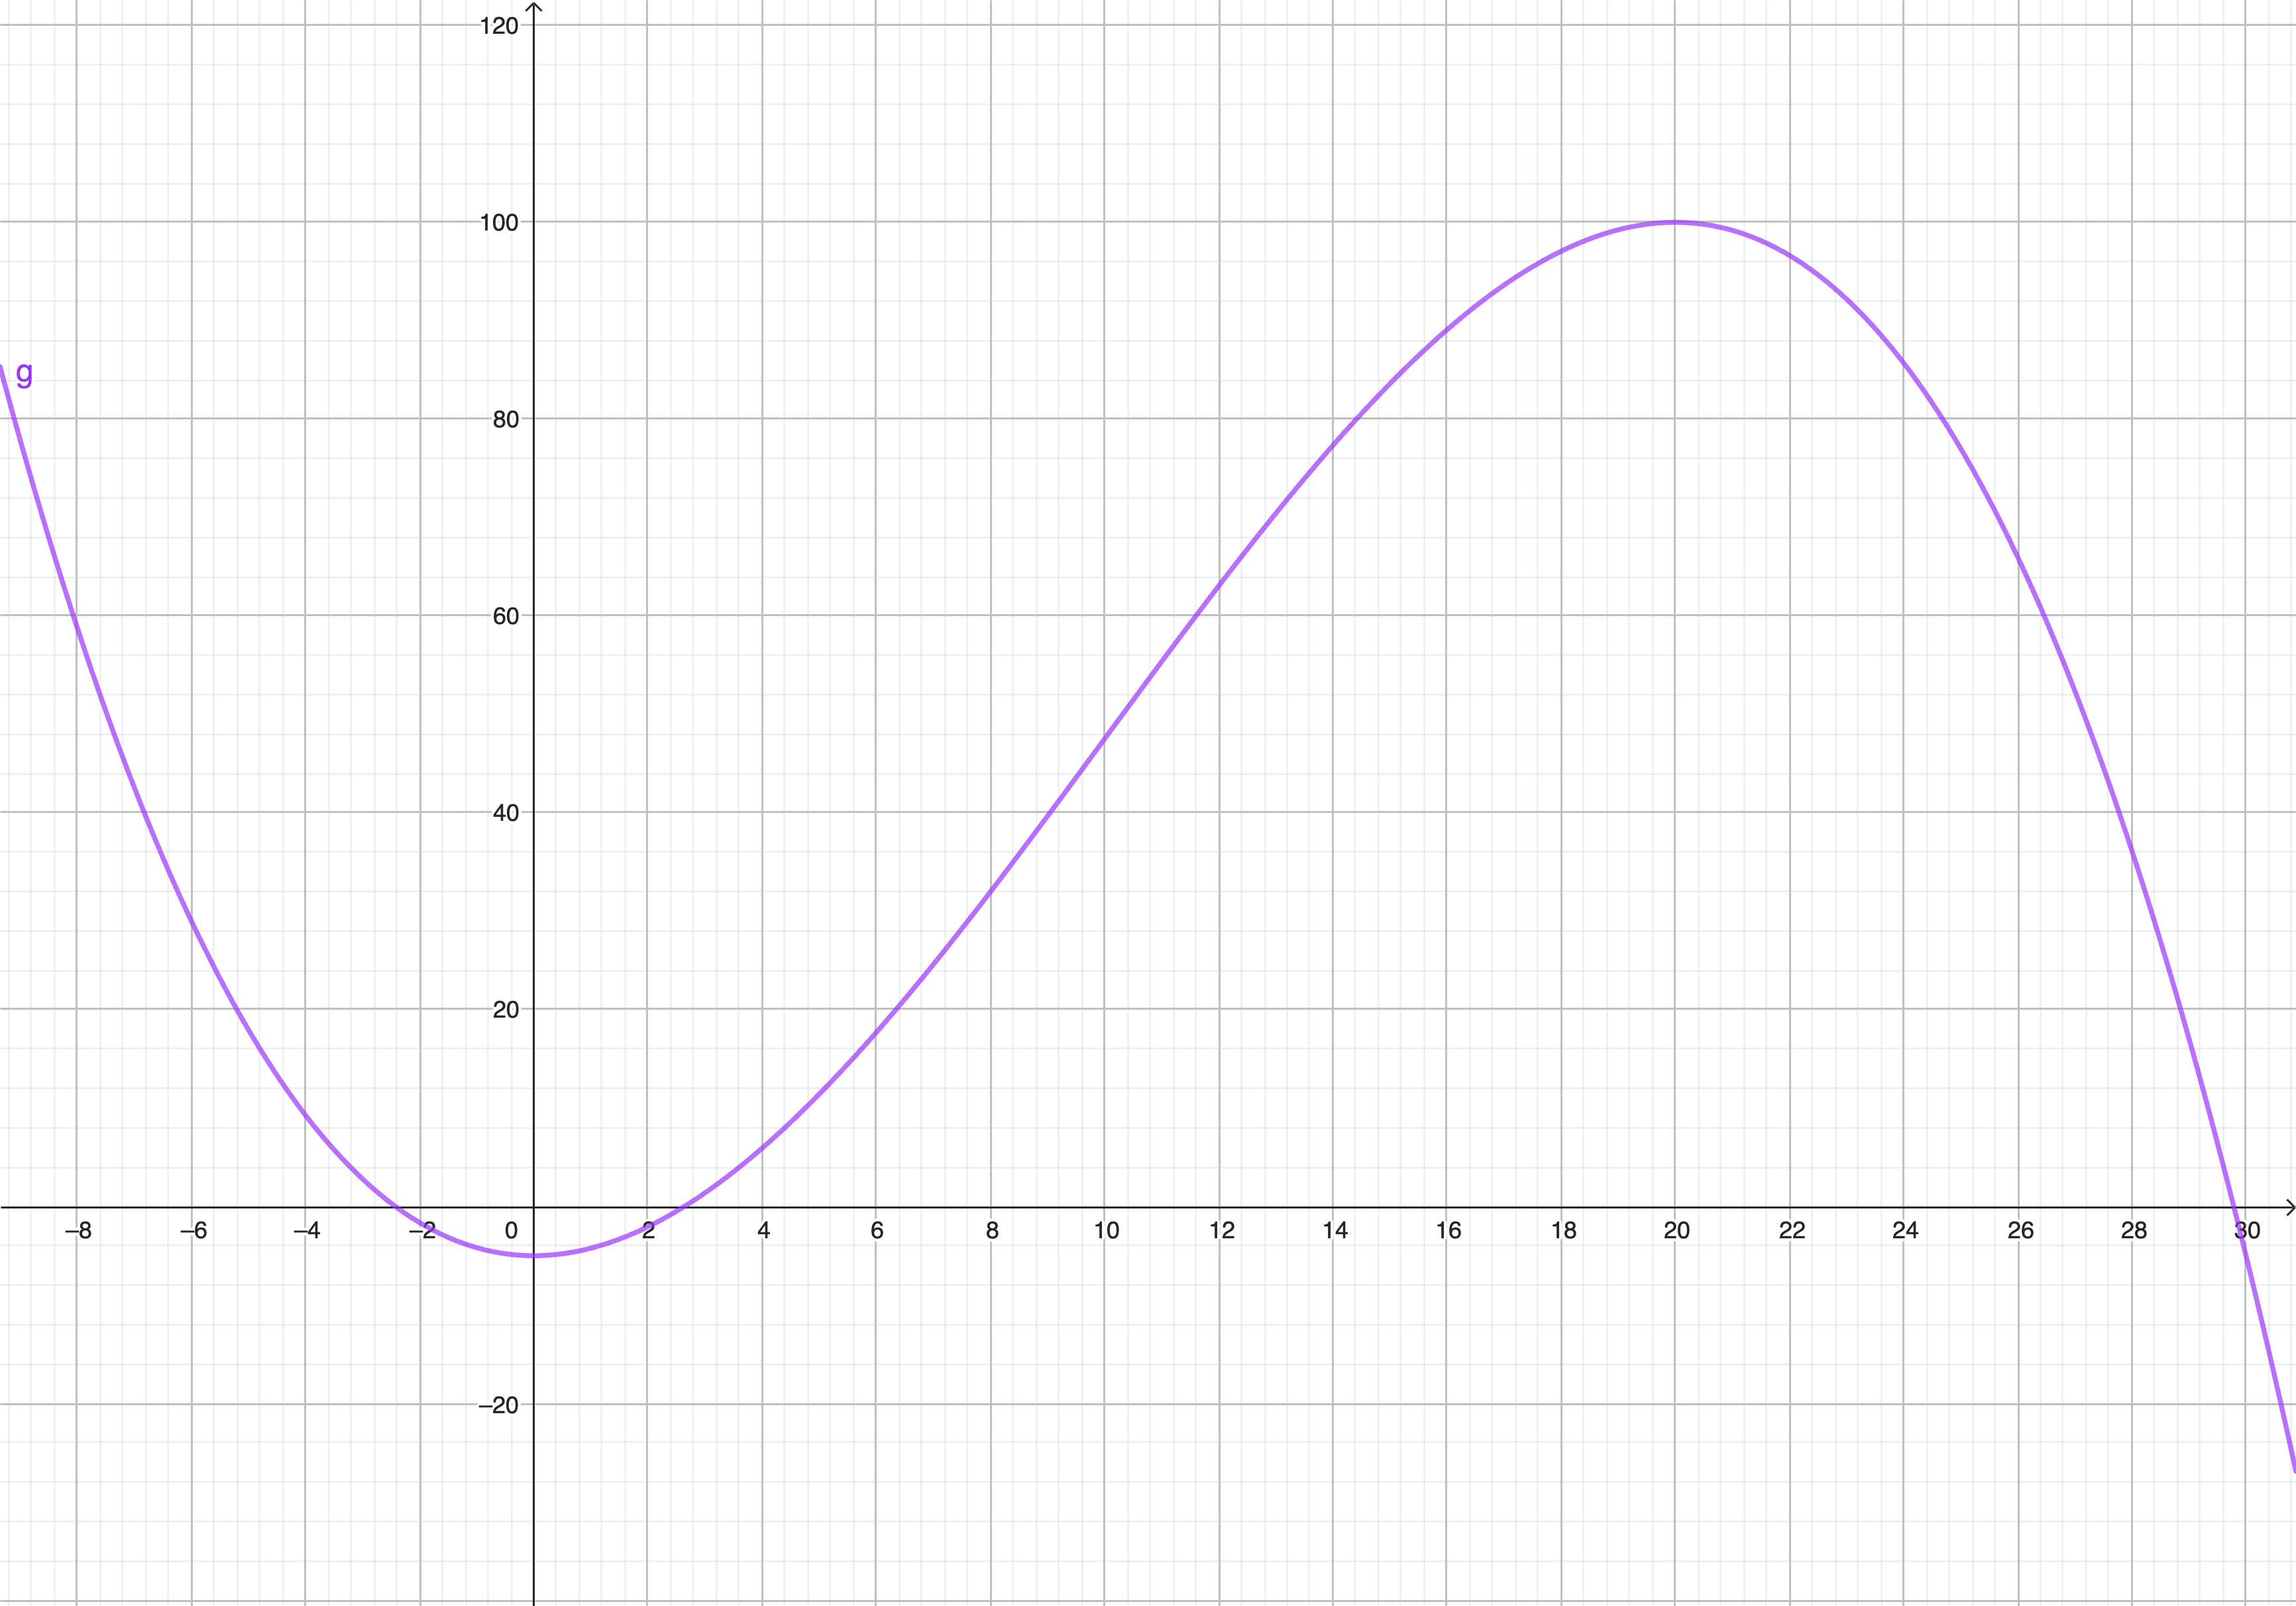
\includegraphics[width=0.7\textwidth]{graf3.png}
\end{figure}
\end{enumerate}

På denne figur kan man se at grafen har vendepunkter i $x=0$ og $x=20$, hvilket også var løsningen til vores ligning fra a). 

\subsection{}
\begin{enumerate}
  \item For at funktionen har netop én rod skal funktionens diskriminant være præcis 0. Bruger vi formlen for diskriminanten med $a=3$, $b=-5$, og $c=c$ kan vi opstille ligningen:
    \begin{align*}
      (-5)^2-4\cdot 3\cdot c&=0\Leftrightarrow\\
      c&=2{,}083
    \end{align*}
    Hvis $c=2{,}083$ har $f$ altså netop én rod.
\end{enumerate}

\end{document}

%%%%%%%%%%%%%%%%%%%%%%%%%%%%%%%%%%%%%%%%%%%%%%%%%%%%%%%%%%%%%%%%%%%%%%%%%%%%%% Skabeloner

% Sidestillet figur
\begin{wrapfigure}[8]{r}{0.2\textwidth}
\vspace{-18pt}
\includegraphics[width=0.3\textwidth]{ovn}
\end{wrapfigure}

% Midterstillet figur
\begin{figure}[H]
\centering
\includegraphics[width=0.8\textwidth]{abc}
\end{figure}

% Førstillet figur
\
\begin{figure}[h!]
\centering
\vspace{-15pt}
\includegraphics[width=0.35\textwidth]{stud}
\end{figure}

% Tabel
\begin{figure}[h!]
\centering\renewcommand{\arraystretch}{1.5}
\begin{tabularx}{0.9\textwidth}{|l|b|b|b|b|b|b|}
	\hline \cellcolor{hggreen} Decimaltal & 7\% & -51\% & 13,7\% & 126\% & 456\% & 0,28\%\\\hline
	\cellcolor{hggreen} Procenttal &  &  &  &  &  & \\\hline
\end{tabularx}
\end{figure}

% Forklaringsopgaver
\begin{align*}
&&	&						&&\underset{\rule{0.8\linewidth}{0pt}}{\textbf{Forklaring:}}\\[1em]
&&	&\frac{(x+2)^2 - 4}{x} 		&&\underset{\rule{0.8\linewidth}{0.4pt}}{\text{Udtrykket skrives op.}}\\[2em]
&&	=&\ \frac{x^2 + 4 + 4x - 4}{x}	&&\underset{\rule{0.8\linewidth}{0.4pt}}{\text{}}\\[2em]
&&	=&\ \frac{x^2 + 4x}{x}			&&\underset{\rule{0.8\linewidth}{0.4pt}}{\text{}}\\[2em]
&&	=&\ x + 4					&&\underset{\rule{0.8\linewidth}{0.4pt}}{\text{}}\\[2em]
\end{align*}

% Sørg for at figur er placeret før et vidst sted
\FloatBarrier




